% Compile with pdflatex or xelatex from the project root.
\documentclass[11pt,a4paper]{article}

\usepackage[margin=1in]{geometry}
\usepackage[T1]{fontenc}
\usepackage[utf8]{inputenc}
\usepackage{graphicx}
\usepackage{booktabs}
\usepackage{tabularx}
\usepackage{array}
\usepackage{amsmath}
\usepackage{amssymb}
\usepackage{float}
\usepackage{xcolor}
\usepackage{caption}
\usepackage{subcaption}
\usepackage{enumitem}
\usepackage{listings}
\usepackage[hidelinks]{hyperref}

\graphicspath{{outputs/figures/}}

\definecolor{codebg}{RGB}{247,248,250}
\definecolor{coderule}{RGB}{220,224,230}
\definecolor{codekw}{RGB}{36,41,46}
\definecolor{codecomment}{RGB}{106,115,125}
\definecolor{accent}{RGB}{23,92,155}

\newcolumntype{Y}{>{\raggedright\arraybackslash}X}
\newcolumntype{C}{>{\centering\arraybackslash}X}

\lstdefinestyle{pythonstyle}{
    language=Python,
    backgroundcolor=\color{codebg},
    basicstyle=\ttfamily\small,
    keywordstyle=\bfseries\color{codekw},
    commentstyle=\itshape\color{codecomment},
    showstringspaces=false,
    breaklines=true,
    frame=single,
    rulecolor=\color{coderule},
    columns=fullflexible
}

\setlist[itemize]{topsep=3pt,itemsep=3pt,leftmargin=1.5em}
\setlength{\parskip}{0.5em}
\setlength{\parindent}{0pt}

\title{\textbf{SS-DBSCAN Project Report}\\[0.4em]
\large A Visual Comparison of DBSCAN and SS-DBSCAN on Three Datasets}
\author{}
\date{April 14, 2026}

\begin{document}

\maketitle

\begin{abstract}
This report presents a three-dataset comparison between standard DBSCAN and the
paper-inspired SS-DBSCAN algorithm. The project is designed so that a reader can
understand the algorithms mainly through figures, cluster plots, runtime graphs,
and compact parameter tables. The experiments use the reference
\texttt{dataset/lettersPreProc.csv}, the Weka dataset
\texttt{dataset/iris.arff}, and a generated synthetic varied-density dataset.
Across the three datasets, the visual results show that SS-DBSCAN changes
cluster expansion by filtering which dense points are allowed to drive growth.
That change is especially helpful on the synthetic dataset, where DBSCAN merges
two blobs into one cluster while SS-DBSCAN recovers the intended two-cluster
structure.
\end{abstract}

\tableofcontents
\clearpage

\section{Simple Algorithm Description}

DBSCAN is a density-based clustering algorithm. The basic intuition is very
simple:

\begin{itemize}
\item A point is \textbf{dense} if many points are close to it.
\item A dense point can act as the center of a cluster.
\item Nearby dense points connect to each other and grow the cluster.
\item Points that are near a cluster but not dense enough themselves become
border points.
\item Points that are not close enough to any cluster are labeled as noise.
\end{itemize}

The key point types are:

\begin{table}[H]
\centering
\small
\begin{tabularx}{\textwidth}{>{\bfseries}lYY}
\toprule
Concept & Intuitive meaning & Practical effect \\
\midrule
Density & How many neighbors lie within a radius $\varepsilon$ & Controls whether a point can support or extend a cluster \\
Core point & A point with enough nearby neighbors & Can start or expand a cluster \\
Border point & A point reachable from a core point but not dense itself & Joins a cluster but does not continue growth \\
Noise & A point not assigned to any cluster & Treated as an outlier \\
\bottomrule
\end{tabularx}
\caption{Core DBSCAN concepts in intuitive form.}
\end{table}

SS-DBSCAN keeps this same density idea but adds one extra filter:
\texttt{Is\_important(point)}. In plain words, SS-DBSCAN asks:

\begin{quote}
``Is this dense point also meaningful enough to continue cluster expansion?''
\end{quote}

That extra rule makes the algorithm semi-supervised. Density still matters, but
the user can inject domain knowledge through the importance condition.

\begin{figure}[H]
\centering
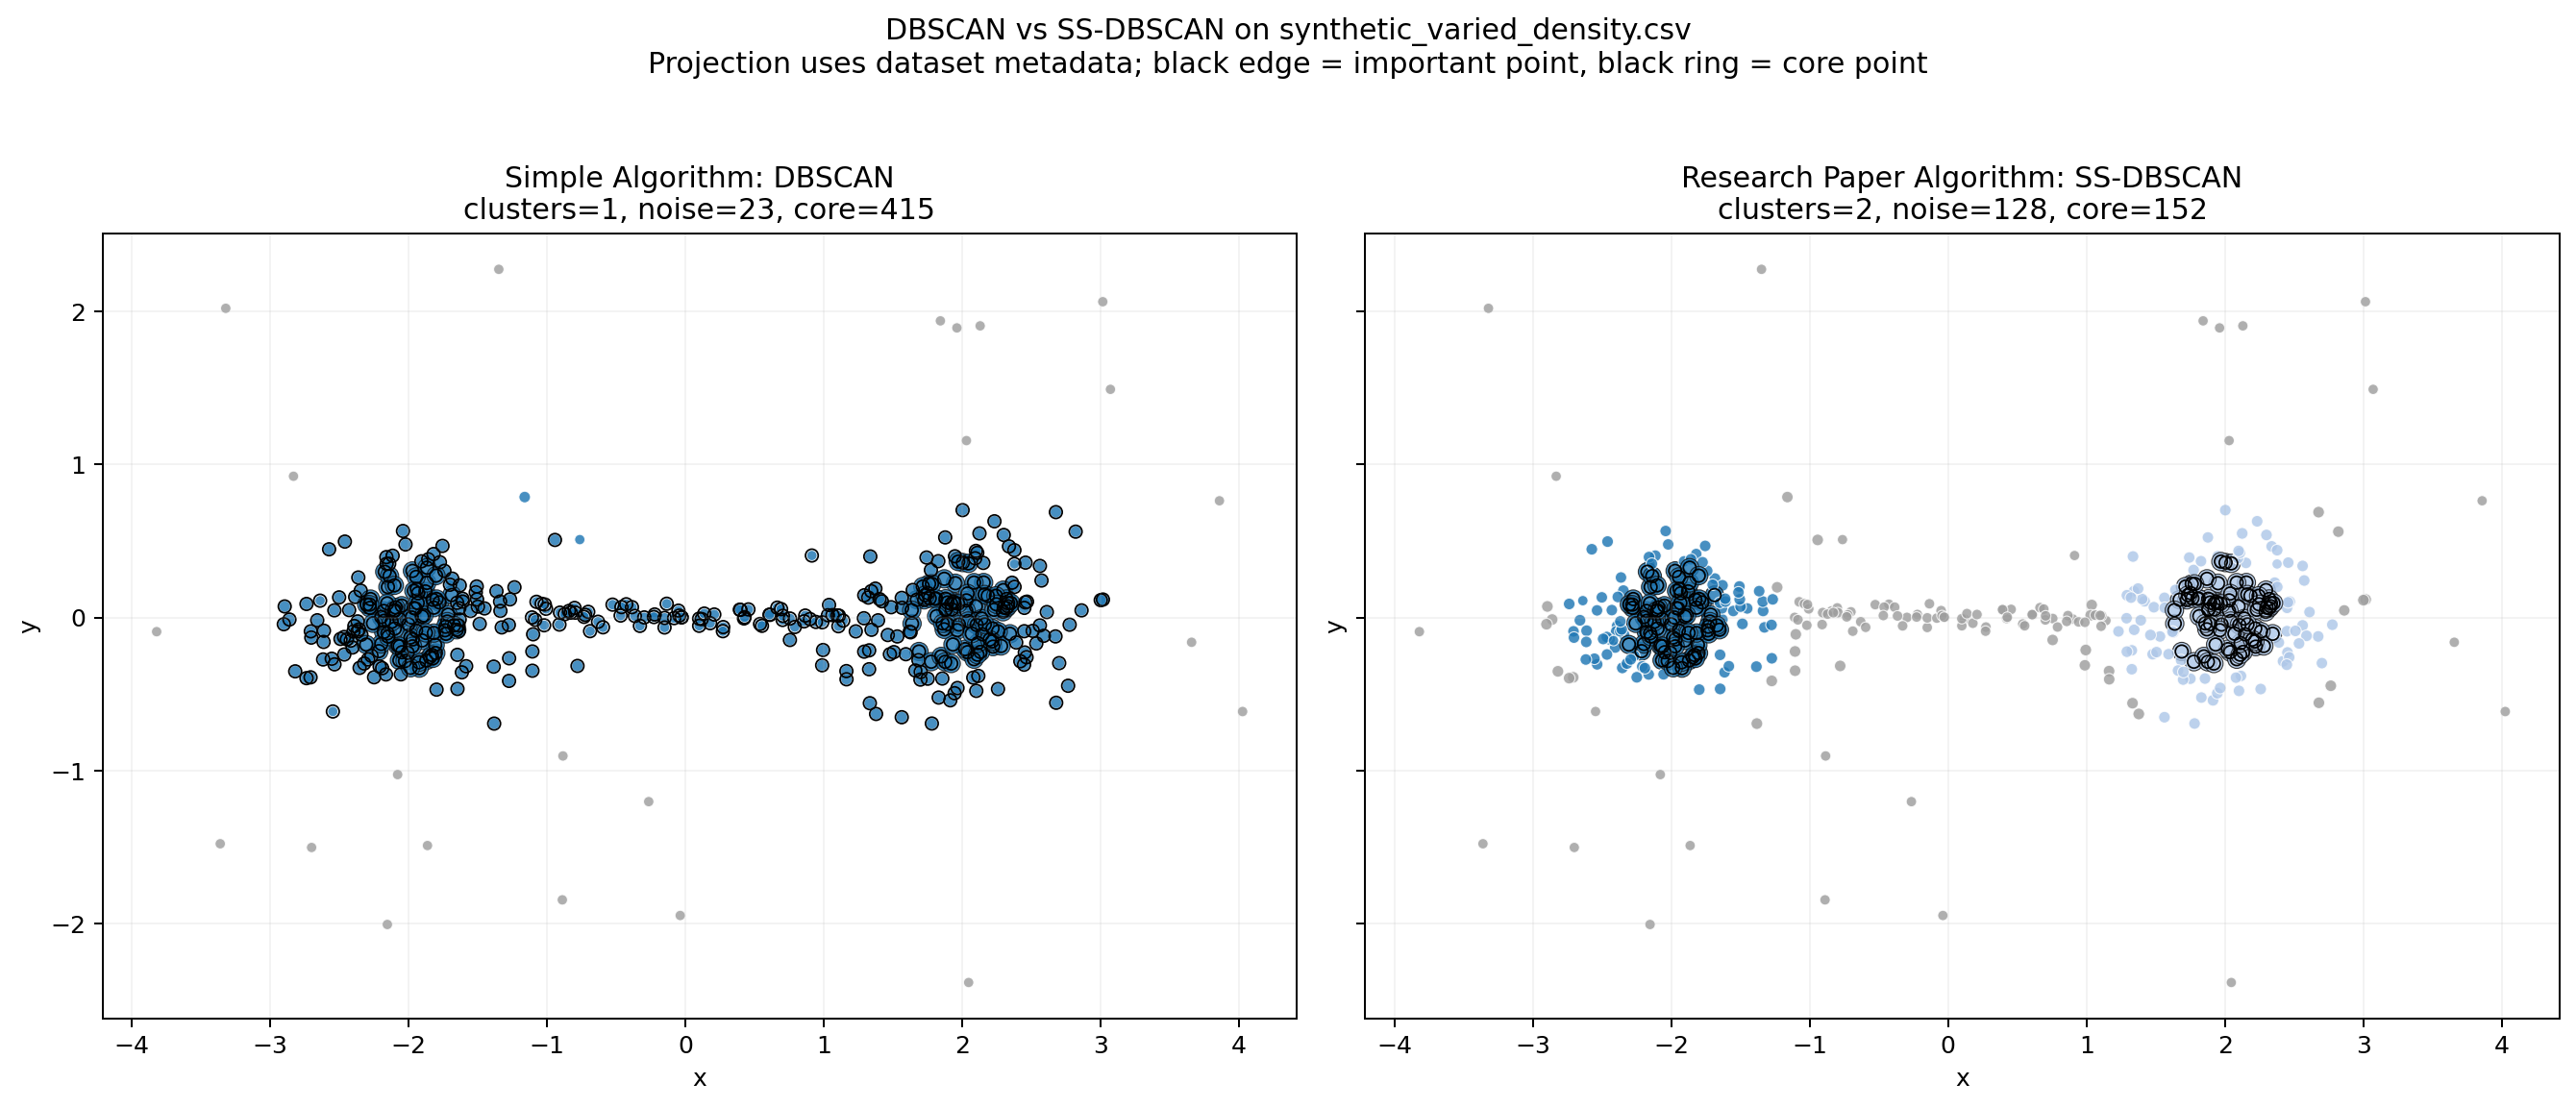
\includegraphics[width=\textwidth]{synthetic_dbscan_vs_ssdbscan.png}
\caption{The synthetic dataset is the easiest visual introduction to the idea.
DBSCAN merges the two dense blobs through the bridge points, while SS-DBSCAN
uses the importance rule to block that incorrect merge and recover two
meaningful clusters.}
\end{figure}

\section{Research Paper Algorithm Description}

\subsection{Formal Density View}

Let the dataset be $D = \{p_1, p_2, \dots, p_n\}$. For a point $p$, its
$\varepsilon$-neighborhood is

\[
N_{\varepsilon}(p) = \{q \in D \mid \operatorname{dist}(p,q) \leq \varepsilon\}.
\]

In standard DBSCAN, a point is considered a core point if

\[
\lvert N_{\varepsilon}(p) \rvert \geq \text{MinPts}.
\]

SS-DBSCAN adds an importance predicate $I(p)$ and uses the condition

\[
\lvert N_{\varepsilon}(p) \rvert \geq \text{MinPts}
\quad \text{and} \quad
I(p)=1.
\]

The project implementation follows the paper idea by using the importance rule
to control cluster expansion. In the synthetic case, important seeds are also
required so that bridge fragments do not become tiny standalone clusters.

\subsection{Step-by-Step Working}

\begin{enumerate}[leftmargin=1.6em]
\item Start with all points unvisited.
\item For each point $p$, compute its neighborhood $N_{\varepsilon}(p)$.
\item If $p$ is not dense enough, mark it as noise and continue.
\item Otherwise, start a new cluster.
\item Expand the cluster using a queue of neighboring points.
\item For every queued point $q$, add it to the cluster.
\item Continue expanding through $q$ only if it is both dense and important.
\item Repeat until no more eligible expansion points remain.
\end{enumerate}

\subsection{Pseudo-code Style Summary}

\begin{lstlisting}[style=pythonstyle,caption={Paper-style clustering logic in simplified pseudo-code.}]
for each unvisited point p:
    neighbors = N_eps(p)

    if len(neighbors) < MinPts:
        label[p] = NOISE
        continue

    create new cluster C
    add p to C
    queue = neighbors

    while queue is not empty:
        q = queue.pop()
        add q to C

        q_neighbors = N_eps(q)
        if len(q_neighbors) >= MinPts and Is_important(q):
            queue.extend(q_neighbors)
\end{lstlisting}

\subsection{Project-Specific Importance Rules}

The same SS-DBSCAN logic is reused across all three datasets, but the
importance rule changes with the dataset:

\begin{itemize}
\item \textbf{Letters}: a point is important when at least one selected feature
is within two units of that feature's maximum.
\item \textbf{Iris}: a point is important when petal length and petal width both
stay inside the 15th--85th percentile band.
\item \textbf{Synthetic}: a point is important when
\texttt{importance\_radius > 2 * mean(importance\_radius)}.
\end{itemize}

\section{Parameters Comparison Table}

\subsection{Algorithm-Level Parameters}

\begin{table}[H]
\centering
\small
\begin{tabularx}{\textwidth}{>{\bfseries}lCCCCY}
\toprule
Parameter & DBSCAN & SS-DBSCAN & Type & Symbol & Effect on clustering \\
\midrule
Neighborhood radius & Yes & Yes & Numeric & $\varepsilon$ & Larger values connect more points and can merge clusters; smaller values split clusters and increase noise \\
Minimum neighbors & Yes & Yes & Integer & MinPts & Larger values make it harder to become a core point; smaller values make clustering easier but can over-connect data \\
Importance rule & No & Yes & Logical rule & $I(p)$ & Filters which dense points can continue expansion, injecting domain knowledge \\
Seed-importance requirement & No & Optional in this project & Boolean & -- & Used for the synthetic dataset so unimportant bridge points do not start their own clusters \\
Distance feature set & Yes & Yes & Column subset & -- & Controls which dimensions define neighborhood distance \\
\bottomrule
\end{tabularx}
\caption{Parameter comparison between the baseline algorithm and the research-paper-based algorithm.}
\end{table}

\subsection{Dataset-Specific Settings Used in This Project}

\begin{table}[H]
\centering
\small
\begin{tabularx}{\textwidth}{>{\bfseries}lCCCCY}
\toprule
Dataset & Rows & Features used for distance & $\varepsilon$ & MinPts & Importance rule \\
\midrule
\texttt{lettersPreProc.csv} & 20,000 & all 16 features & 8.0 & 17 & selected features near their maximum \\
\texttt{dataset/iris.arff} & 150 & all 4 numeric features & 0.9 & 4 & petal features inside a percentile band \\
\texttt{synthetic\_varied\_density.csv} & 440 & \texttt{x}, \texttt{y} & 0.45 & 5 & high importance radius \\
\bottomrule
\end{tabularx}
\caption{The exact settings used in the verified current run.}
\end{table}

\section{Graphical Comparison}

This section is intentionally visual. The goal is that a reader can understand
the project without reading every equation first.

\subsection{Cluster Visualizations}

\begin{figure}[H]
\centering
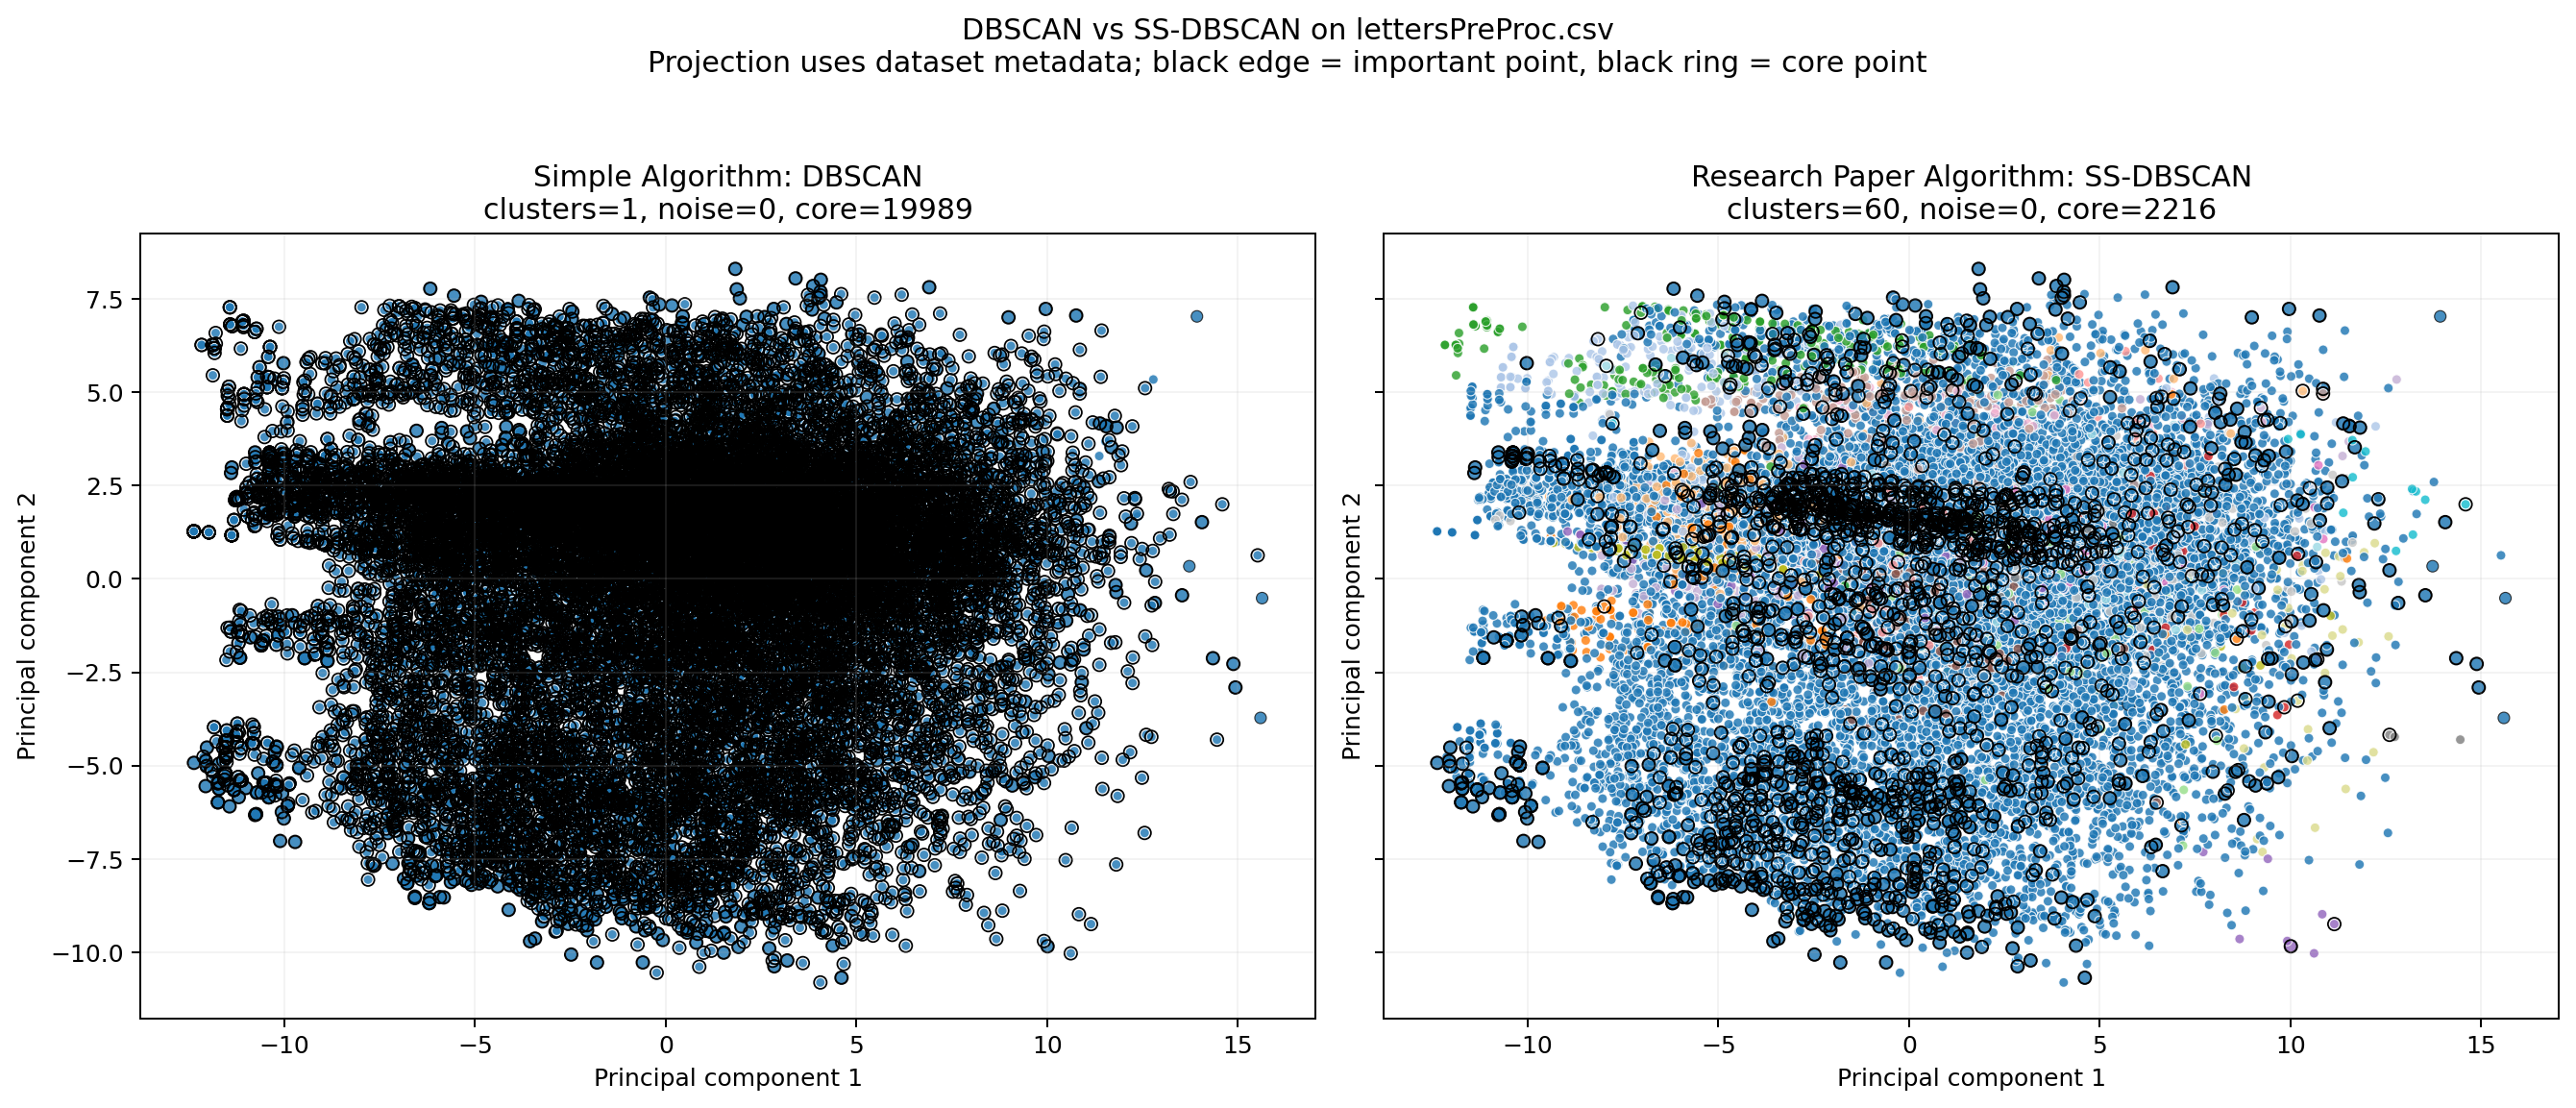
\includegraphics[width=\textwidth]{letters_dbscan_vs_ssdbscan.png}
\caption{Cluster comparison on \texttt{lettersPreProc.csv}. The left panel shows
that DBSCAN collapses the dataset into one cluster. The right panel shows that
SS-DBSCAN becomes much more selective when the importance rule is applied.}
\end{figure}

\begin{figure}[H]
\centering
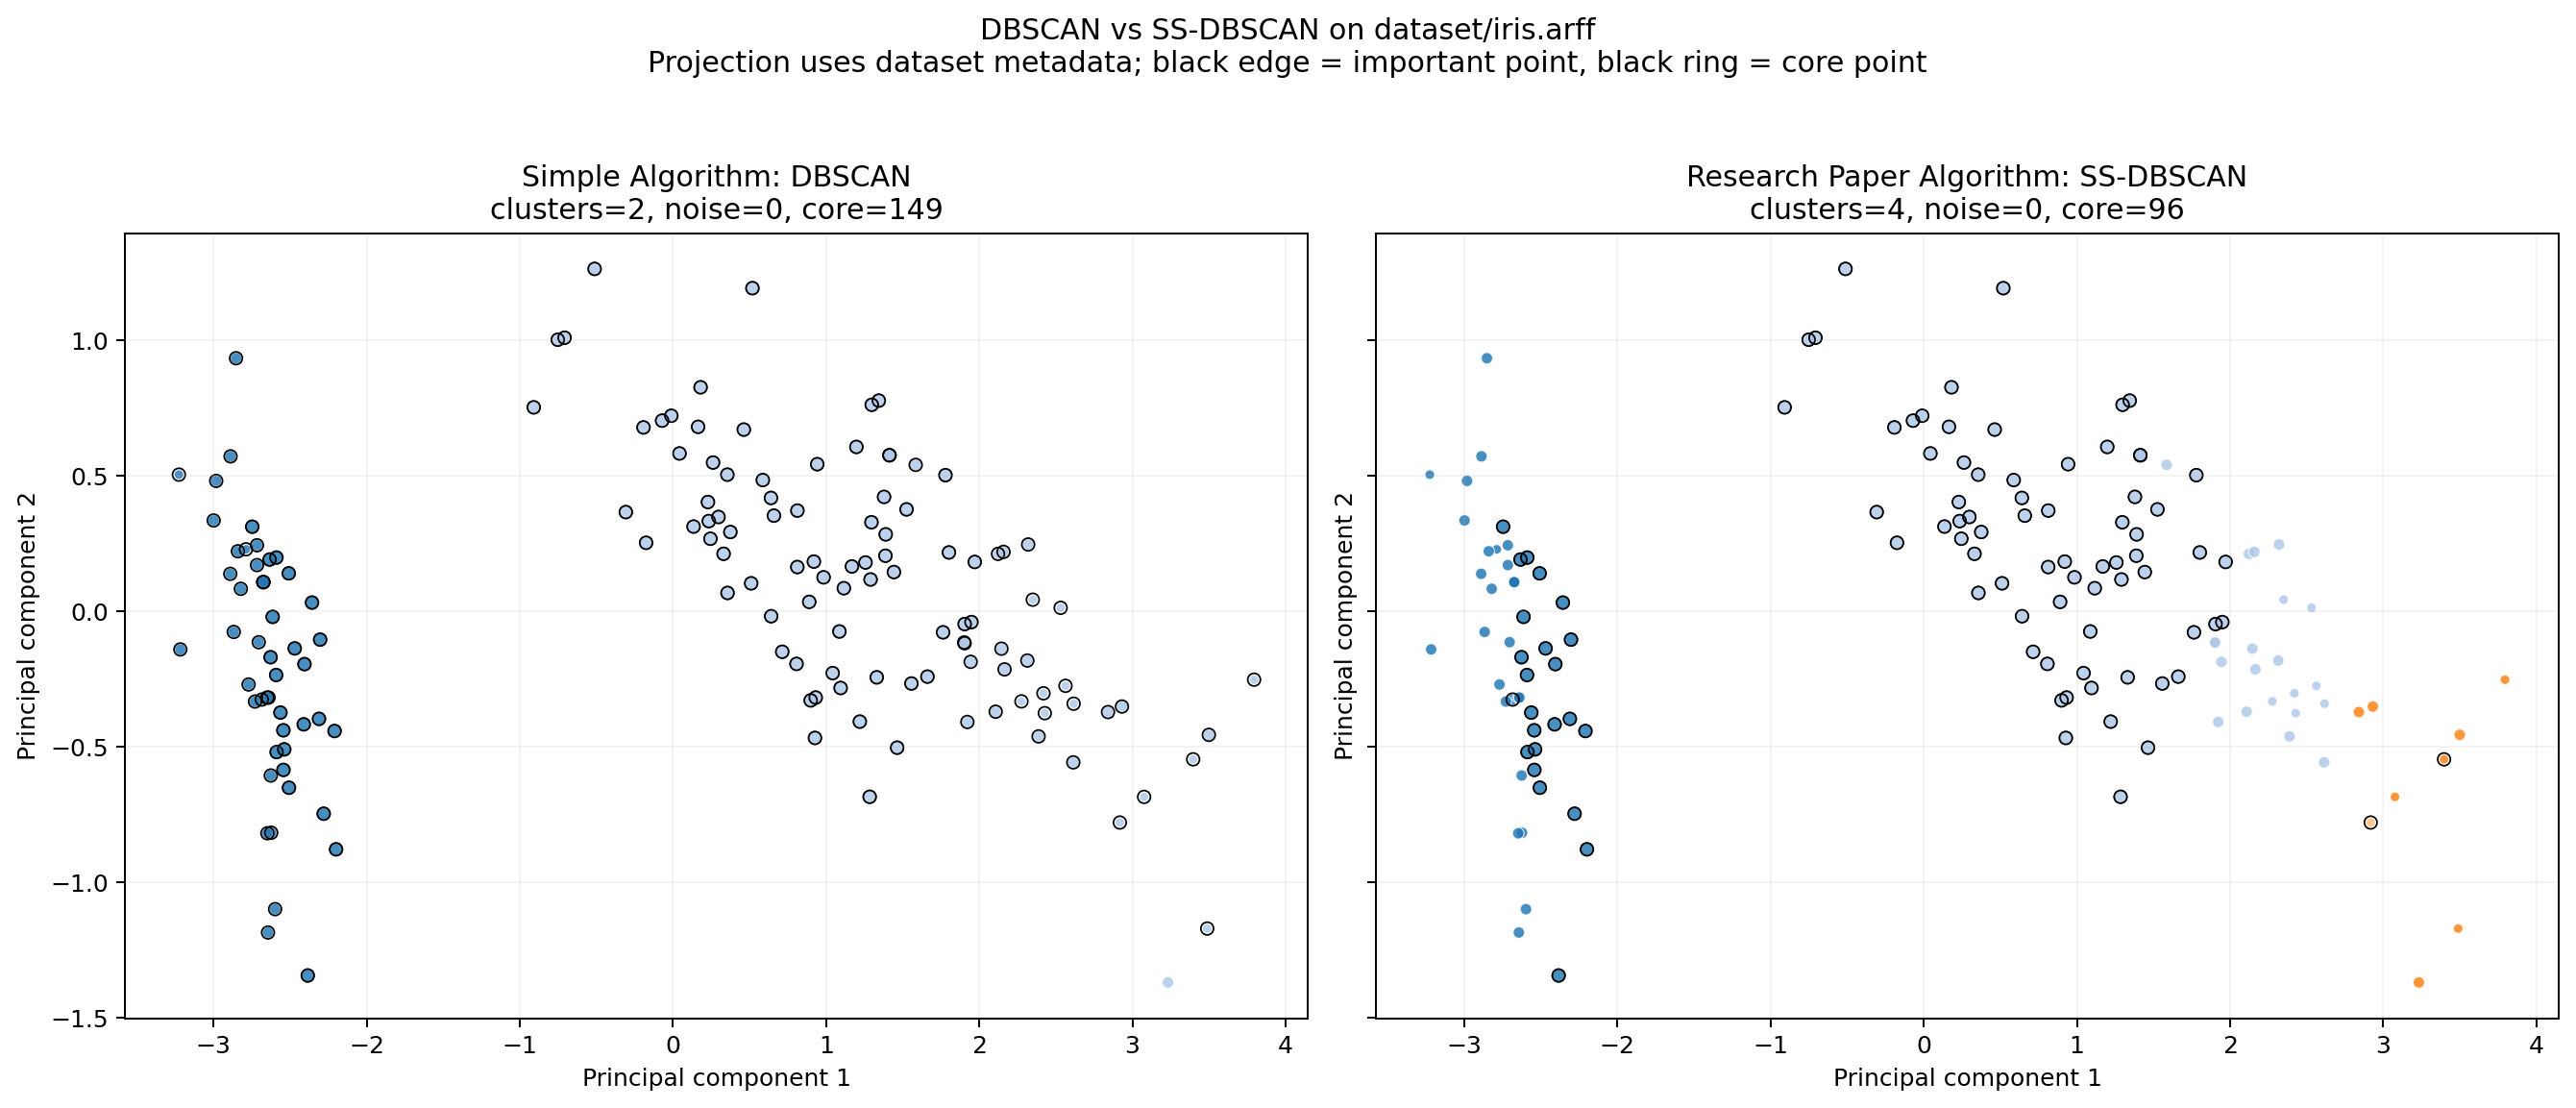
\includegraphics[width=\textwidth]{iris_dbscan_vs_ssdbscan.png}
\caption{Cluster comparison on \texttt{dataset/iris.arff}. Here DBSCAN and
SS-DBSCAN produce different cluster structures, but both stay reasonably close
in clustering quality.}
\end{figure}

\begin{figure}[H]
\centering
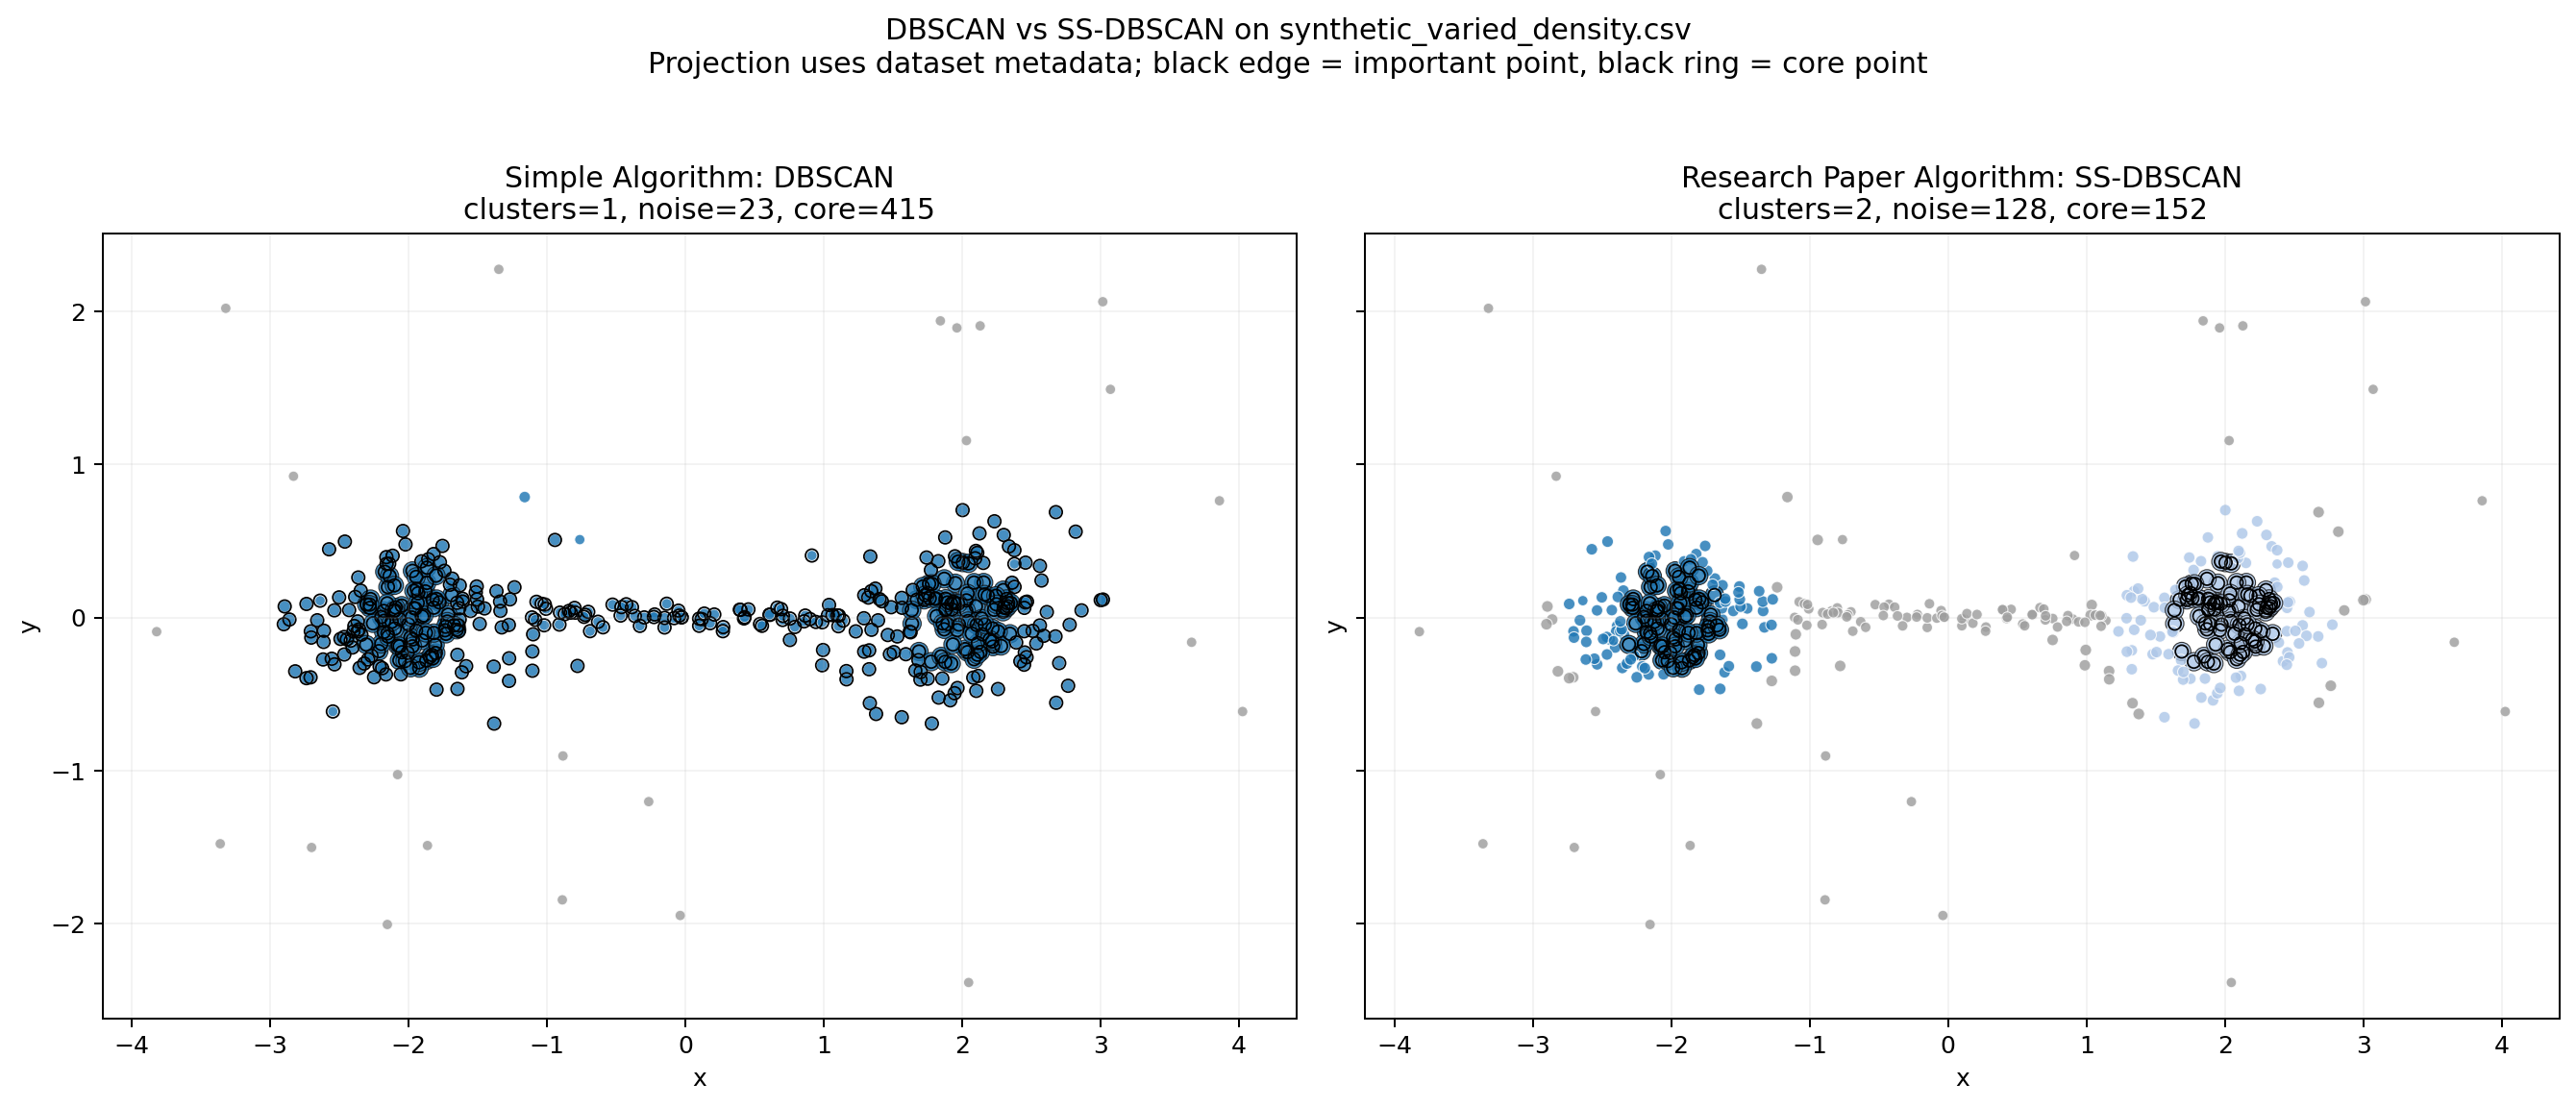
\includegraphics[width=\textwidth]{synthetic_dbscan_vs_ssdbscan.png}
\caption{Cluster comparison on the generated synthetic dataset. This is the
cleanest visual example of the intended SS-DBSCAN behavior.}
\end{figure}

\subsection{Quality Summary Table}

\begin{table}[H]
\centering
\small
\begin{tabularx}{\textwidth}{>{\bfseries}l>{\bfseries}lCCCCCC}
\toprule
Dataset & Algorithm & Clusters & Noise & Core points & V-measure & ARI & Runtime (s) \\
\midrule
Letters & DBSCAN & 1 & 0 & 19,989 & 0.0000 & 0.0000 & 20.563980 \\
Letters & SS-DBSCAN & 60 & 0 & 2,216 & 0.1488 & 0.0042 & 13.936038 \\
Iris & DBSCAN & 2 & 0 & 149 & 0.7337 & 0.5681 & 0.001998 \\
Iris & SS-DBSCAN & 4 & 0 & 96 & 0.6958 & 0.5592 & 0.001525 \\
Synthetic & DBSCAN & 1 & 23 & 415 & 0.1294 & 0.0525 & 0.012078 \\
Synthetic & SS-DBSCAN & 2 & 128 & 152 & 0.7605 & 0.7977 & 0.009416 \\
\bottomrule
\end{tabularx}
\caption{Visual figures are backed by the quantitative results from the latest verified run.}
\end{table}

\subsection{What the Reader Should Notice}

\begin{itemize}
\item \textbf{Letters}: DBSCAN is too permissive with the reference settings and
merges almost everything.
\item \textbf{Iris}: both algorithms are reasonable, but the SS filter changes
the structure rather than clearly dominating the baseline.
\item \textbf{Synthetic}: SS-DBSCAN shows the intended improvement most clearly,
because the bridge points are no longer allowed to drive expansion.
\end{itemize}

\section{Python Implementation}

The Python project implements both algorithms through one shared clustering
engine and switches behavior by changing the importance rule.

\subsection{Public Algorithm Entry Points}

\begin{lstlisting}[style=pythonstyle,caption={Public DBSCAN and SS-DBSCAN entry points used in the project.}]
def dbscan(data, *, eps, min_pts, distance_columns=(0, 1)):
    return _density_clustering(
        data,
        eps=eps,
        min_pts=min_pts,
        distance_columns=distance_columns,
        importance_rule=lambda _point, _index: True,
        require_seed_importance=True,
    )

def ss_dbscan(
    data,
    *,
    eps,
    min_pts,
    importance_rule,
    distance_columns=(0, 1),
    require_seed_importance=False,
):
    return _density_clustering(
        data,
        eps=eps,
        min_pts=min_pts,
        distance_columns=distance_columns,
        importance_rule=importance_rule,
        require_seed_importance=require_seed_importance,
    )
\end{lstlisting}

\subsection{How Input Data Is Processed}

\begin{itemize}
\item The runner loads or generates each dataset.
\item Each dataset defines which columns are used for distance.
\item An importance profile is computed per dataset.
\item DBSCAN runs with the rule ``all dense points are allowed''.
\item SS-DBSCAN runs with the dataset-specific importance rule.
\end{itemize}

\begin{lstlisting}[style=pythonstyle,caption={Dataset configuration used by the three-experiment runner.}]
ExperimentConfig(
    dataset_id="letters",
    loader=lambda: load_letters_dataset(LETTERS_DATASET_PATH),
    importance_profile_builder=compute_letters_importance_profile,
    eps=8.0,
    min_pts=17,
    require_seed_importance=False,
)

ExperimentConfig(
    dataset_id="iris",
    loader=lambda: load_iris_dataset(IRIS_DATASET_PATH),
    importance_profile_builder=compute_iris_importance_profile,
    eps=0.9,
    min_pts=4,
    require_seed_importance=False,
)

ExperimentConfig(
    dataset_id="synthetic",
    loader=_load_synthetic_dataset,
    importance_profile_builder=None,
    eps=0.45,
    min_pts=5,
    require_seed_importance=True,
)
\end{lstlisting}

\subsection{How Clusters Are Formed}

\begin{lstlisting}[style=pythonstyle,caption={The expansion rule where SS-DBSCAN differs from baseline DBSCAN.}]
current_neighbors = neighbor_graph[point_index]
is_core = len(current_neighbors) >= min_pts and importance_rule(
    data[point_index],
    point_index,
)

if not is_core:
    continue

core_mask[point_index] = True
for neighbor_index in current_neighbors:
    if neighbor_index not in queued:
        queue.append(neighbor_index)
\end{lstlisting}

The important idea is that the same queue-based cluster growth exists in both
algorithms. The difference is that SS-DBSCAN only lets selected dense points
keep the growth going.

\section{Code + Theory Integration}

\begin{table}[H]
\centering
\small
\begin{tabularx}{\textwidth}{>{\bfseries}lYY}
\toprule
Theory statement & Where it appears in code & Meaning in practice \\
\midrule
$N_{\varepsilon}(p)$ defines local density & \texttt{\_build\_neighbor\_graph(...)} & Precomputes which points are within the chosen neighborhood radius \\
Core-point test depends on MinPts & \texttt{len(neighbors) >= min\_pts} & Implements the standard DBSCAN density condition \\
SS-DBSCAN adds user knowledge & \texttt{importance\_rule(data[point\_index], point\_index)} & Lets each dataset decide which dense points are meaningful \\
Synthetic seed control avoids bridge fragments & \texttt{require\_seed\_importance=True} & Produces the intended 1-vs-2 visual comparison on the synthetic data \\
Experiment design is dataset-specific & \texttt{ExperimentConfig(...)} & Keeps one common algorithm but changes rules and parameters per dataset \\
\bottomrule
\end{tabularx}
\caption{Direct mapping from theory to implementation.}
\end{table}

\subsection{Integration Narrative}

\begin{itemize}
\item Theoretical density is translated into an epsilon-neighborhood graph.
\item The MinPts rule becomes a direct count test on each neighborhood.
\item The paper's semi-supervised idea becomes a Python callback:
\texttt{importance\_rule}.
\item The synthetic experiment adds an implementation-level safeguard so
unimportant bridge points do not start tiny clusters.
\end{itemize}

\section{Theoretical Differences}

\begin{table}[H]
\centering
\small
\begin{tabularx}{\textwidth}{>{\bfseries}lYY}
\toprule
Aspect & Simple algorithm (DBSCAN) & Research-paper algorithm (SS-DBSCAN) \\
\midrule
Core idea & Density alone determines cluster growth & Density plus importance determines cluster growth \\
Human knowledge & Not used & Explicitly used through \texttt{Is\_important(point)} \\
Behavior in bridge regions & Can connect clusters through dense bridges & Can block expansion through unimportant bridge points \\
Behavior in sparse regions & Often increases noise or fragmentation when parameters are strict & Depends on how importance interacts with sparse points \\
Interpretability & Easier to explain as one density rule & More expressive because domain knowledge is visible in the rule design \\
Edge cases & Sensitive to global density settings & Sensitive to both density settings and quality of the importance rule \\
\bottomrule
\end{tabularx}
\caption{Conceptual differences between the baseline method and the research-paper method.}
\end{table}

\subsection{Dataset-Specific Interpretation}

\begin{itemize}
\item On \textbf{letters}, the SS rule changes behavior strongly, but the chosen
reference settings still do not align well with the ground-truth classes.
\item On \textbf{iris}, the SS rule changes structure without creating a dramatic
quality improvement over the baseline.
\item On the \textbf{synthetic} dataset, the SS rule successfully handles the
bridge region and preserves the intended two-cluster interpretation.
\end{itemize}

\section{Time Complexity Analysis (Computation)}

\subsection{Asymptotic View}

For both algorithms, the dominant cost comes from neighborhood computations. In
the worst case:

\[
T_{\text{DBSCAN}}(n) = O(n^2),
\qquad
T_{\text{SS-DBSCAN}}(n) = O(n^2).
\]

The project does \emph{not} store one huge dense distance matrix for the
largest dataset. Instead, it computes epsilon-neighborhoods in chunks. This
changes the practical memory footprint, but the worst-case time behavior stays
quadratic.

\[
S_{\text{worst case}} = O(n^2)
\]

in dense-neighborhood situations, although the chunked implementation is much
friendlier in practice than building one full distance matrix at once.

\subsection{Runtime Graphs}

\begin{figure}[H]
\centering
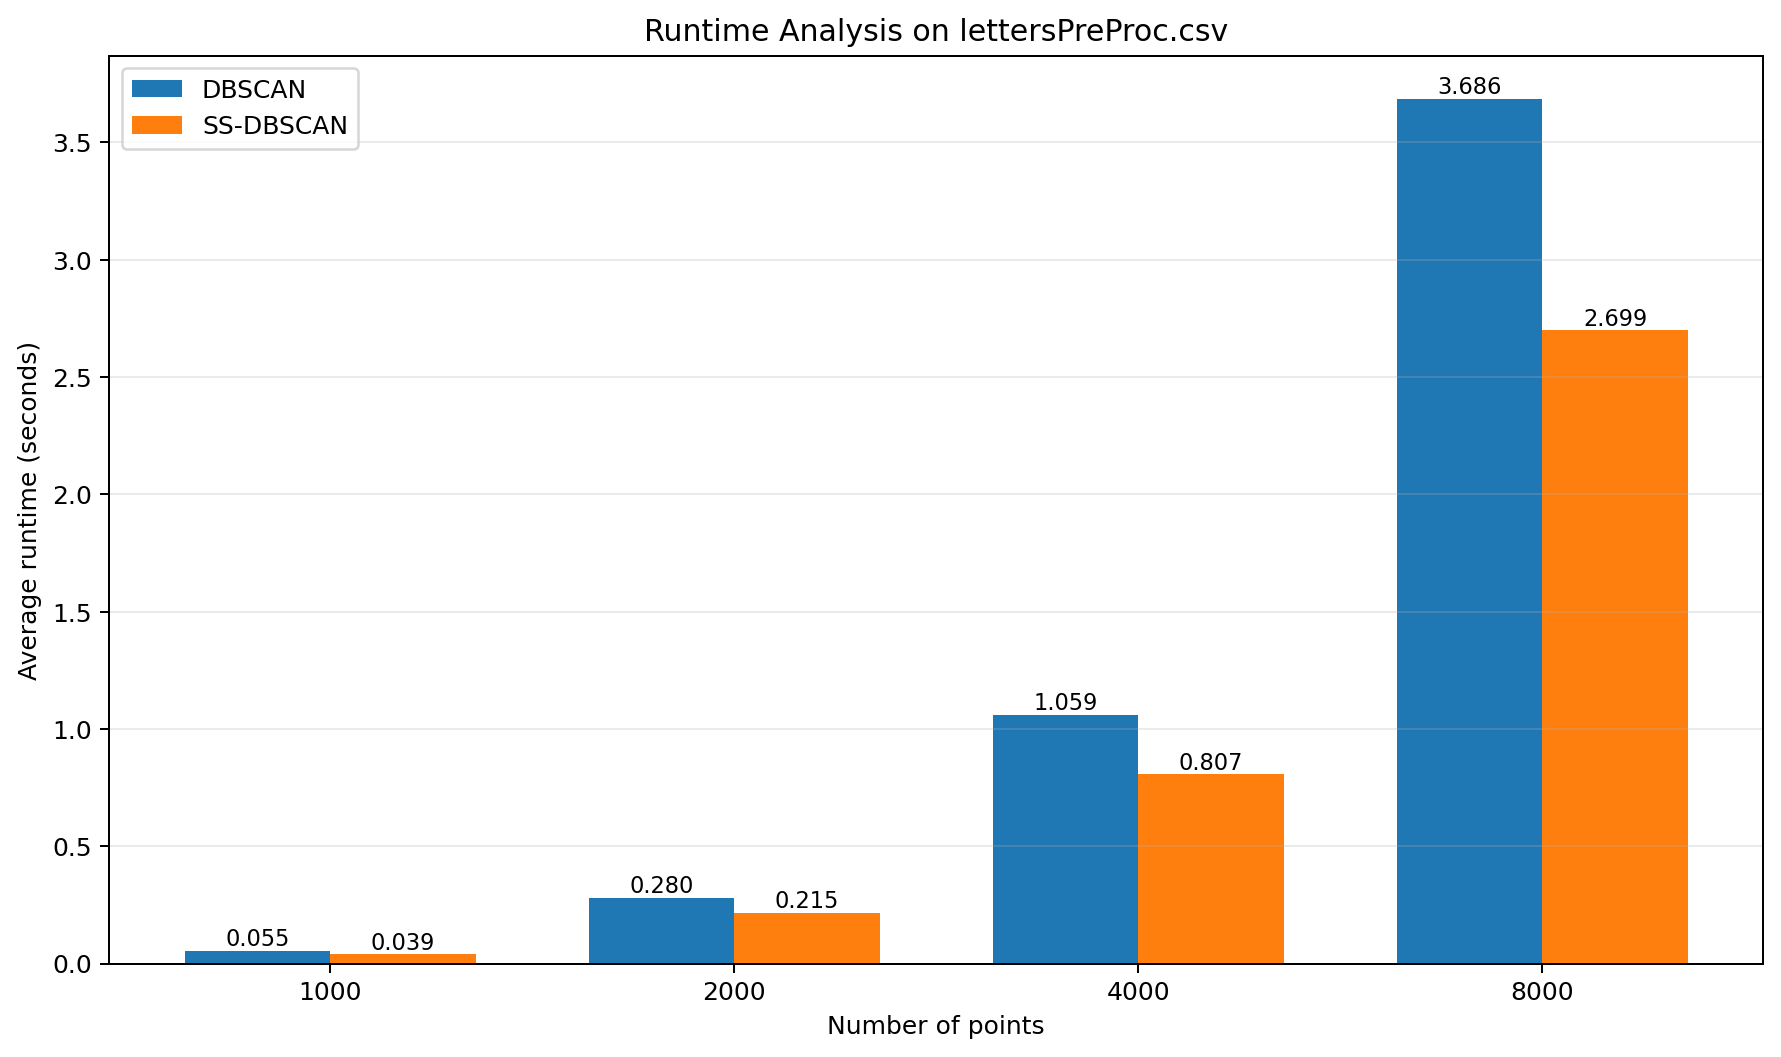
\includegraphics[width=\textwidth]{letters_runtime_comparison.png}
\caption{Runtime comparison on \texttt{lettersPreProc.csv} subsets.}
\end{figure}

\begin{figure}[H]
\centering
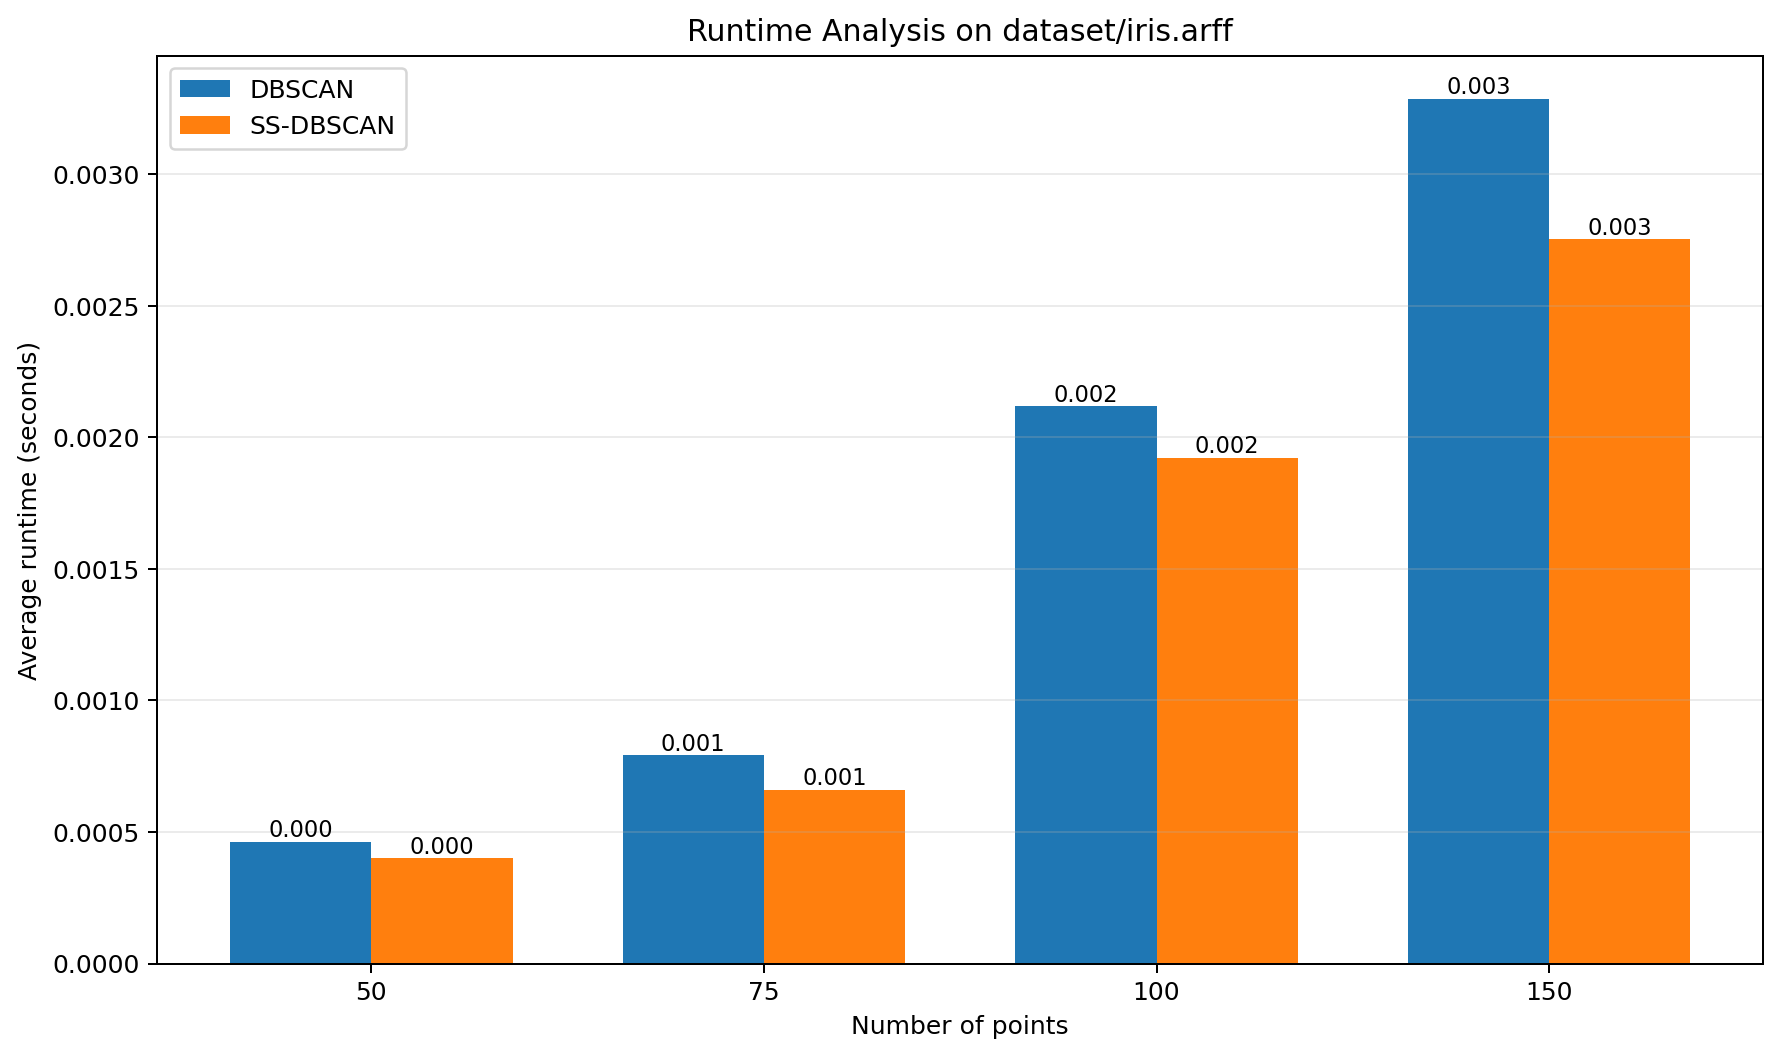
\includegraphics[width=\textwidth]{iris_runtime_comparison.png}
\caption{Runtime comparison on \texttt{dataset/iris.arff}.}
\end{figure}

\begin{figure}[H]
\centering
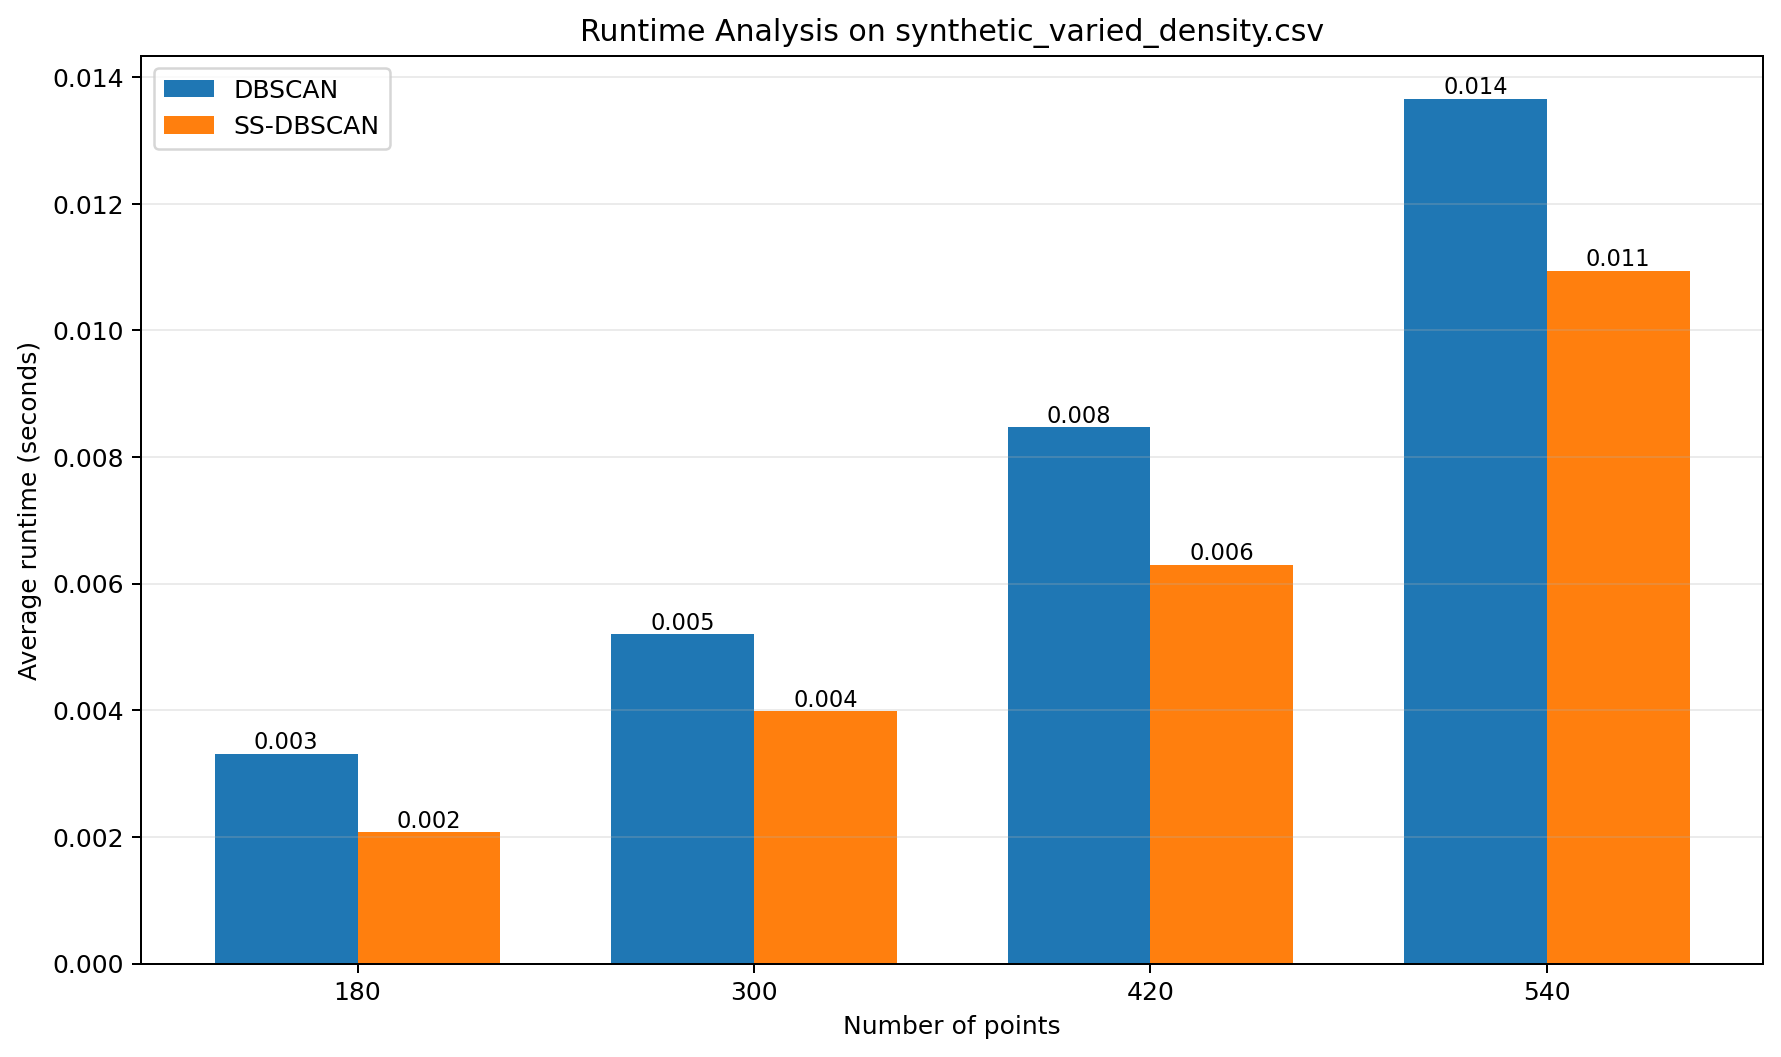
\includegraphics[width=\textwidth]{synthetic_runtime_comparison.png}
\caption{Runtime comparison on the generated synthetic dataset.}
\end{figure}

\subsection{Runtime Summary Tables}

\begin{table}[H]
\centering
\small
\begin{tabular}{rcc}
\toprule
Points & DBSCAN (s) & SS-DBSCAN (s) \\
\midrule
\multicolumn{3}{c}{\textbf{Letters}} \\
1,000 & 0.055356 & 0.038859 \\
2,000 & 0.280042 & 0.215297 \\
4,000 & 1.059117 & 0.806675 \\
8,000 & 3.685767 & 2.698778 \\
\midrule
\multicolumn{3}{c}{\textbf{Iris}} \\
50 & 0.000463 & 0.000400 \\
75 & 0.000791 & 0.000661 \\
100 & 0.002118 & 0.001923 \\
150 & 0.003286 & 0.002753 \\
\midrule
\multicolumn{3}{c}{\textbf{Synthetic}} \\
180 & 0.003312 & 0.002072 \\
300 & 0.005201 & 0.003982 \\
420 & 0.008467 & 0.006299 \\
540 & 0.013655 & 0.010939 \\
\bottomrule
\end{tabular}
\caption{Measured runtime summaries used by the project report.}
\end{table}

\subsection{Why One Can Be Faster}

SS-DBSCAN is sometimes slightly faster in this project because the importance
rule reduces the number of points that are allowed to continue expansion. In
other words, the extra logical condition can reduce the amount of queue growth
even though it adds one more check per candidate point.

\section*{Conclusion}

This project report was intentionally built around visualization. The cluster
plots and runtime figures make the main story easy to see:

\begin{itemize}
\item DBSCAN is a strong baseline, but it can over-merge data when density alone
is not expressive enough.
\item SS-DBSCAN adds a user-defined importance rule, which changes which dense
points are allowed to shape the cluster structure.
\item The synthetic dataset shows the cleanest success case for SS-DBSCAN.
\item The letters and iris datasets show that the value of SS-DBSCAN depends on
how well the importance rule matches the structure of the data.
\end{itemize}

\end{document}
